\section{Results and Discussion}

The classification results for the features extracted from the functional connectivity maps are shown in Fig. \ref{fig:kappa}. Higher kappa values indicate better classification performance. A kappa value $k=0$ indicates a random decision. According to Figure \ref{fig:kappa}, a higher classification performance is achieved with Nonlinear Regression Analysis (NRA) compared to Granger's Causality (GC). One-way \emph{Student-t test} was applied to test the significance of non-randomness. The null hypothesis is that the kappa values for each case follow a Student distribution with zero mean. The NRA results sucessfully passed the test with $p<0.05$ (with $\kappa$ value $\mu = 0.06, \sigma = 0.14$, 14 out of 23 subjects have kappa values larger than zero). The null hypothesis is not rejected for the GC case. The higher kappa values from NRA network classifiers indicate that nonlinear patterns occur in the functional connectivity of neural assemblies, who able to discriminate between pleasantness and unpleasantness during olfactory perceptions. 

\begin{figure}[t]
    \centering
    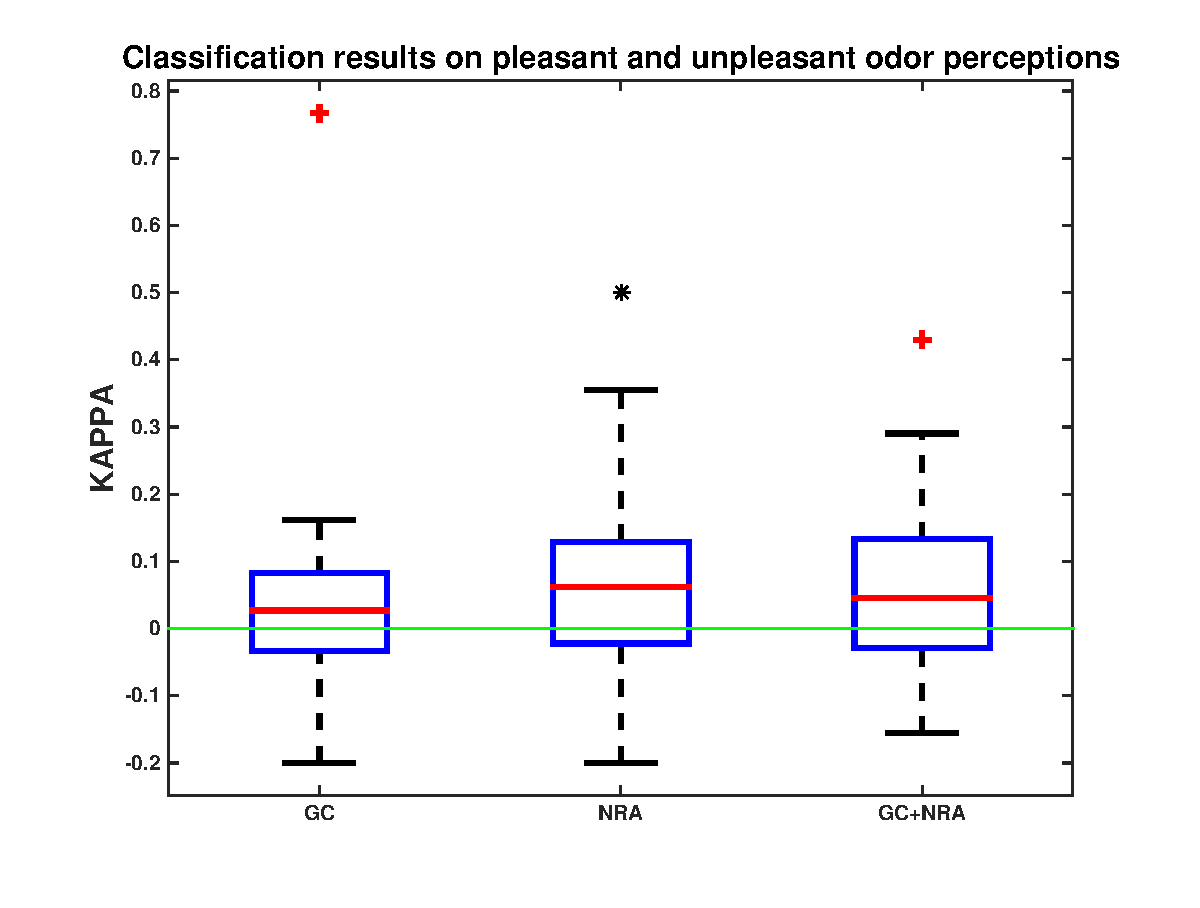
\includegraphics[width=0.45\textwidth]{./images/kappa.eps}
    \caption{Cohen's Kappa results boxplots. On each box, the central (red) line represents the median value, the upside and downside edges represent the 25th and 75th percentiles, and the red crosses represent outliers. The green line represents the random decision, $Kappa=0$. GC refers to the kappa values estimated for features extracted from the functional connectivity maps estimated using Granger Causality. NRA refers to the kappa values estimated for features extracted from the maps estimated using Nonlinear Regression Analysis. GC+NRA refers to the kappa values estimated using features both from Granger Causality and from Nonlinear Regression Analysis.}
    \label{fig:kappa}
\end{figure}

%%%%%%%%%%%%%%%%%%%%%%%%%%%%%%%%%%%%%%%%%%%%%%%%%%%%%%%%%%%%%%%%%%%%%%%%%%%%%%
%%                             TABLE 1
%%%%%%%%%%%%%%%%%%%%%%%%%%%%%%%%%%%%%%%%%%%%%%%%%%%%%%%%%%%%%%%%%%%%%%%%%%%%%%
\begin{table}[ht]
\caption{Kappa descriptives for each classification scenario. Min stands for minimum kappa value, max for maximum kappa value, and SD for standard deviation. One asterisk indicates significance with $p<0.05$, and two asterisks with $p<0.01$.}\label{Table1}
\centering % for placing the table in the middle of the page
{\begin{tabular}{|l|c|c|c|c|}
\hline
\toprule
 \textbf{Features} & \textbf{Min} & \textbf{Max} & \textbf{Mean} & \textbf{SD} \\
\hline
\toprule
\textbf{GC} & -0.2 & 0.77 & 0.07 & 0.23 \\
\hline
\toprule
 \textbf{NRA*} & -0.2 & 0.19 & 0.06 & 0.14 \\
\hline
\toprule
\textbf{GC+NRA*} & -0.07 & 0.18 & 0.05 & 0.08  \\
\hline
\toprule
\textbf{NRA(Characteristic path**)} & -0.1 & 0.45 & 0.096 & 0.15 \\
\hline
\toprule
\textbf{NRA(Local efficiency**)} & -0.14 & 0.37 & 0.09 & 0.14 \\
\hline
\toprule
\textbf{NRA(Global efficiency**)} & -0.17 & 0.5 & 0.11 & 0.17 \\
\hline
\toprule
 \textbf{NRA(Clustering coefficient**)} & -0.15 & 0.5 & 0.11 & 0.16 \\
\hline
\toprule
\textbf{NRA(Shannon entropy)} & -0.13 & 0.34 & 0.07 & 0.12 \\
\hline
\toprule
\textbf{NRA(von Neumann entropy)} & -0.13 & 0.3 & 0.01 & 0.12 \\
\bottomrule
\end{tabular}}
%\begin{tabnote}
%SD indicates Significant Differences (with $p<0.01$), whereas NS indicates No Significant differences ($p>0.05$).
%\end{tabnote}
\end{table}
%%%%%%%%%%%%%%%%%%%%%%%%%%%%%%%%%%%%%%%%%%%%%%%%%%%%%%%%%%%%%%%%%%%%%%%%%%%%%%

%In order to investigate the classification performance of the two feature-categories, namely the small-world network features and the free-scale network features, a SVM classifier is trained and tested as previously, for each feature-category. The results are presented in Table \label{Table1}. In order to investigate if each feature-category leads to significantly non-random kappa values, a one-way \emph{Student-t test} is applied as previously. The results reveal that the small-world network features lead to a significantly non-random performance, whereas this is not the case for the free-scale network features. This finding indicates that odor pleasantness perception can be depicted in small-world network features extracted from the functional connectivity across neural assemblies which is estimated using Nonlinear Regression Analysis. 
%
%
%Finally, in order to further explore which individual feature increases the classification performance, the same analysis as previously is carried out for each feature. The results are also presented in Table \lref{Table1}. According to this table, all small-world network features lead to a similar classification performance, which is significantly non-random ($p<0.01$). 
The most representative kappa descriptives are summarised in Table \ref{Table1}. \textbf{GC} represents the network features (both small-world and scale-free types) extracted from Linear Granger Causality functional connectivity network. \textbf{NRA} represents the network features (both small-world and scale-free types) extracted from Nonlinear Regression Analysis functional connectivity network. \textbf{GC+NRA} represents the combined network features from both functional connectivity networks. Since the NRA network gives a better kappa performance, we further investigated the classification performance of each single network feature of the NRA functional connectivity network, using the same scenario of classification and statistical tests as described in previous sections. The results reveal that the small-world network features (characteristic path, local efficiency, global efficiency and clustering coefficient) have a better classification performance compared to scale-free network features. This result indicates that odor pleasantness perception can be depicted in small-world network features extracted from the functional connectivity across neural assemblies which is estimated using Nonlinear Regression Analysis. 

Additionally, free-scale networks are known for their property of self-similarity in finer scales. However, in our case free-scale network features did not lead to significantly non-random results, indicating that self-similar properties of functional connectivity maps may not be responsible for odor pleasantness discrimination. 

However, the best obtained accuracy ($0.11 \pm 0.17$), although significantly non-random, is not very high. Compared with previous study on olfactory pleasantness perception using other methods such as power spectral density~\cite{kroupi2014eeg}, our results are not outstanding. We expect that by integrating information from the brain functional connectivity with commonly used features for odor pleasantness perception (such as power spectral density features), the classification performance can be improved. 

This work in analyzing network features from functional connectivity networks in general can have a great impact in affective computing. The method we had proposed in this paper can help revealing additional knowledge about how information flows during underlying emotional processes. Due to the limitations of research on odors (still many questions open regarding exposition time, etc.), it would be very interesting to further explore if similar patterns occur and if the classification performance is increased using more conventional affective stimuli, such as video and audio.   


%Although the significant kappa result have a $p-values$ less than 0.05, some of the $p-values$ are still very close to 0.05, indicating that the results are not that good anyway.The low classification accuracy may due to many reasons: the size of functional connectivity map may play a crucial rule in classification -- the 216-channel functional connectivity maps may provide too much redundant information in classification. New features of functional connectivity maps should also be proposed and used for classification. Since we only used network-based features in this paper, other features as power spectral density or time-frequency analysis may also be used in combination for classification. Another improvement for getting better classification results could be done in the experiment design. Based on the experiment protocol and preprocessing of raw EEG signal, 6 seconds of each trial of EEG signal are kept fro investigating the pleasantness from odors. This time duration could be cut shorter (because 6 seconds might be to much for decision making) or extended longer (or because 6 seconds might be not enough to make the decision). Nevertheless, this paper is not targeting to replace existing methods for affective computing on emotions, but to propose a new direction for affective computing. 